\section{Network architecture}

\subsection{IoT networks}

\begin{itemize}
		\item Interconnectivity of all things
		\item Extremely heterogenous network
		\item Permanent changes to topology
		\item Large scale
\end{itemize}

\subsubsection{Architecture}

\begin{description}
		\item[Applications] In open networks
		\item[Internet of things] Network + platform + content + objects,
				communicating with applications
\end{description}

\subsection{CPS systems}

\begin{itemize}
		\item Real-time requirements
		\item Control and computing in one devices
		\item Sensor nodes at border of cyber and physical world.
\end{itemize}

\subsubsection{Architecture}

\begin{description}
		\item[Application layer] Containing smart home, smart city, ...
				applications. Security via E2E encryption, intrustino
				detection, user authentication, ...
		\item[Transmission layer] WiFi, bluetooth, ..., connecting devices to
				each other and to applications. Security via robust routnig
				protocols, hop-to-hop encryption, network access control, ...
		\item[Perception layer] Sensors, RFID, actuators, .... Security via key
				agreement, trust management, access control, ...
\end{description}

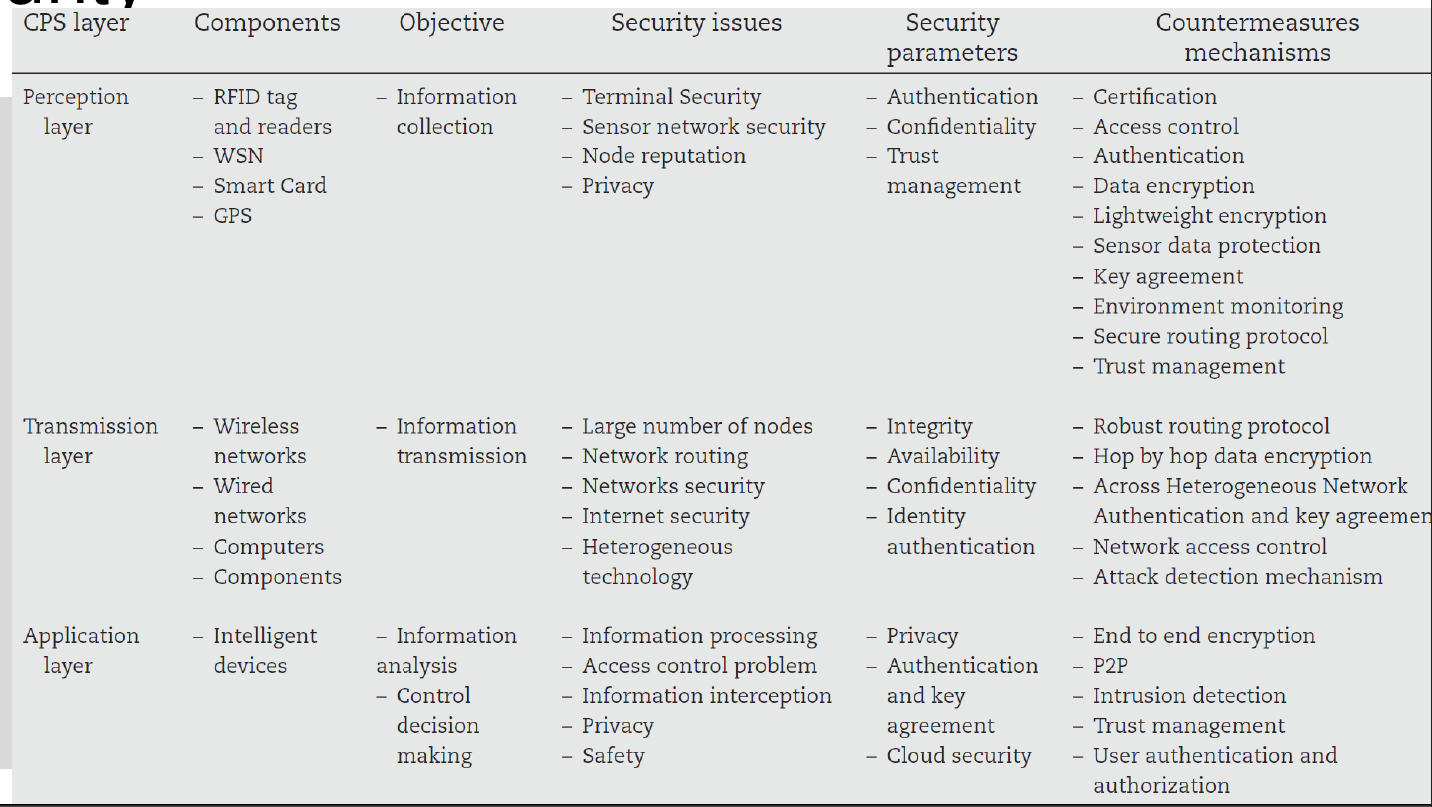
\includegraphics[width=\textwidth]{12_cps}

\subsection{M2M networks}

\begin{itemize}
		\item M2M devices attached to assets of interest, providing sensing and actuation
		\item Network connects M2M devices and application servers
\end{itemize}

\subsubsection{Vs IoT}

\begin{itemize}
		\item Point-problem driven vs innovation driven
		\item Asset-management vs data and information
		\item Closed vs open marketplace
		\item Specialized vs commodity hardware
		\item Proprietary vs open standards
\end{itemize}

\subsubsection{Architecture}

\begin{description}
		\item[Application domain] Application servers and client applications
		\item[Network domain] M2M core, satellite, radio, wired networking
		\item[M2M device domain] M2M devices, connected to network domain via
				M2M gateway, using e.g. wireless M2M area networks
\end{description}

\paragraph{ETSI M2M functional architecture}

\begin{itemize}
		\item Access and core network by mobile network operator (MNO)
		\item IP-based connection (WAN) to applications
		\item Authentication configuration (eg DHCP) built-in
		\item Network domain vs device and gateway domain»
\end{itemize}

\subsection{The Things Network}

\subsubsection{Architecture}

\begin{itemize}
		\item LoraWAN between IoT devices and gateway
		\item Decentralized.
				\begin{itemize}
						\item Nodes talk with gateways
						\item Gateways to one router each
						\item Routers schedule transmissions and manage
								gateway, forward messages to (and receive from)
								brokers
						\item Brokers route upstream to correct application,
								downstream to correct router.
						\item Handlers connect to brokers and receive
								application's data, handle
								encryption/decryption, communicate with
								application via MQTT
						\item Discovery servers allow routers, brokers and
								handles to find each other.
						\item Network servers manage Lorawan specifics
				\end{itemize}
\end{itemize}

\subsubsection{Security}

\begin{itemize}
		\item 128-bit security, E2E encryption
		\item Network session key (NWSKey) for interaction between node and
				network server, e.g. verify validity of message and map
				non-unique device address to unique device ID and app ID
		\item Application session key (AppSKey) for encryption and decryption
				of payload, encrypted between node and handler/application
				server.
		\item Both keys unique per device and session
\end{itemize}

\subsection{Narrowband IoT}

\begin{itemize}
		\item Subset of LTE for IoT devices
		\item Faster than Lorawan (througput \& latency) but higher deployment
				cost and lower range
		\item Used in e.g. utility metering, building automation, industrial
				control, logistics, pet tracking, ...
\end{itemize}

\subsubsection{Architecture}

\begin{itemize}
		\item Devices communicate with core network via access point.
		\item Both command/response, periodic reporting as well as event-based
				reporting possible
		\item Built atop LTE evoled packet system (LTE EPS), optimized for
				cellular IoT, optimizations for user and control plane
\end{itemize}

\subsubsection{Operation modes}

\begin{description}
		\item[In-band] NB-IoT carrier within LTE carrier, using unused LTE
				physical resource blocks (PRB)
		\item[Guard-band] NB-IoT carrier located within guard band of LTE
				(unused band between two LTE bands). Avoids interference,
				better downlink throughput.
		\item[Standalone] Usag of dedicated spectrum
\end{description}

\subsubsection{Frame structure}

\begin{itemize}
		\item Downlink equal to LTE. Radio frame split into 10 subframes of
				\SI{1}{\milli\second} each. Each frame split into 2 slots with
				7 OFDM symbols.
		\item Uplink uses resource grid with subcarrier spacing
\end{itemize}

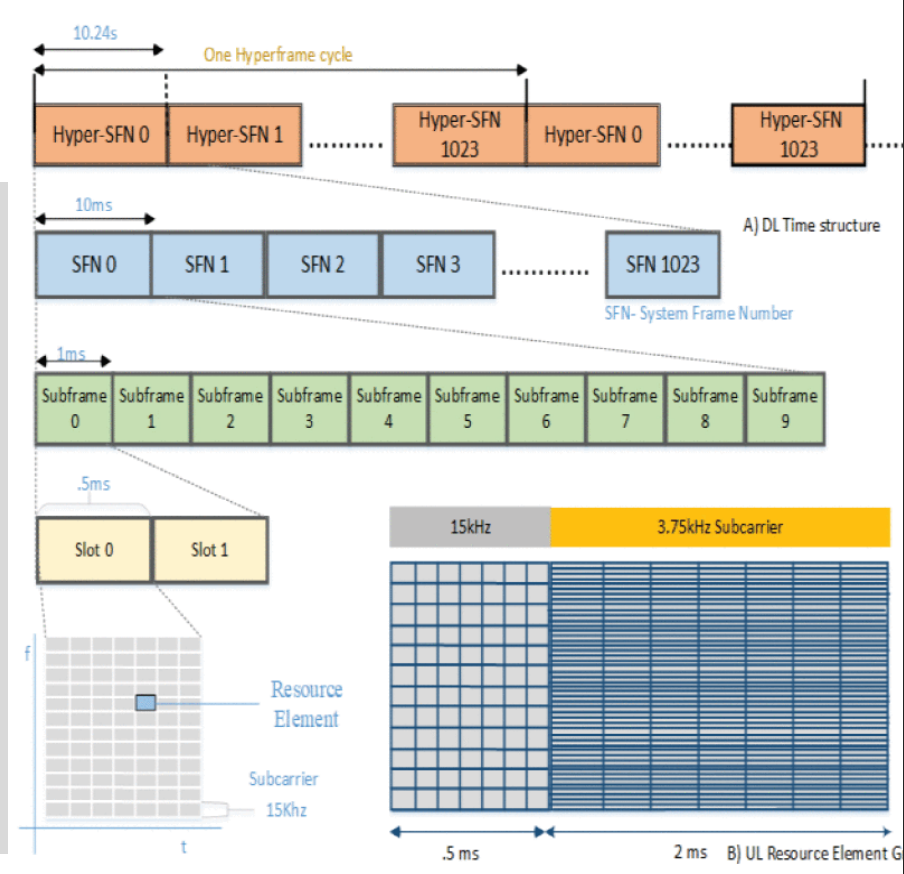
\includegraphics[width=\textwidth]{12_nbiot}

\subsubsection{Physical channels and signals}

\begin{description}
		\item[NPRACH] Narrowband physical random access channel, uplink
		\item[NPUSCH] Narrowband physical uplink shared channel
		\item[DMRS] Demodularion reference signal, multiplexed with NPUSCH
		\item[NBPBCh] Narrow-band physical broadcast channel, downlink,
				carries information on system bandwith etc
		\item[NPDCCh] Narrow-band physical downlink control channel, contains
				scheduling information etc
		\item[NPDSCh] Narrow-band physical downlink shared channel, contains data
		\item[DL synchronization signals] Allow device to synchronize
\end{description}

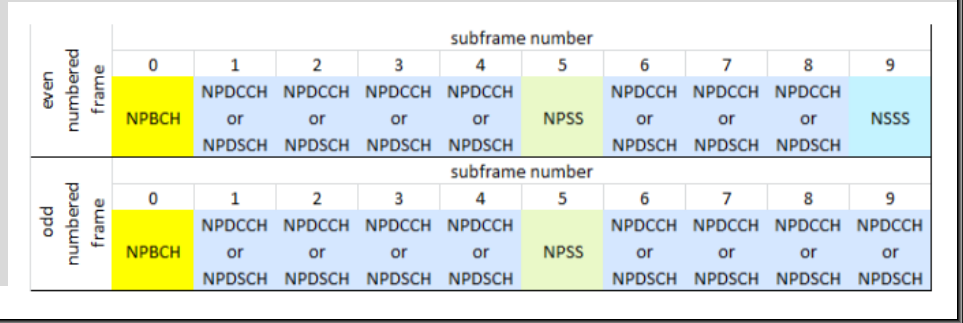
\includegraphics[width=0.5\textwidth]{12_nbiot_channels}

\subsubsection{Transport channels}

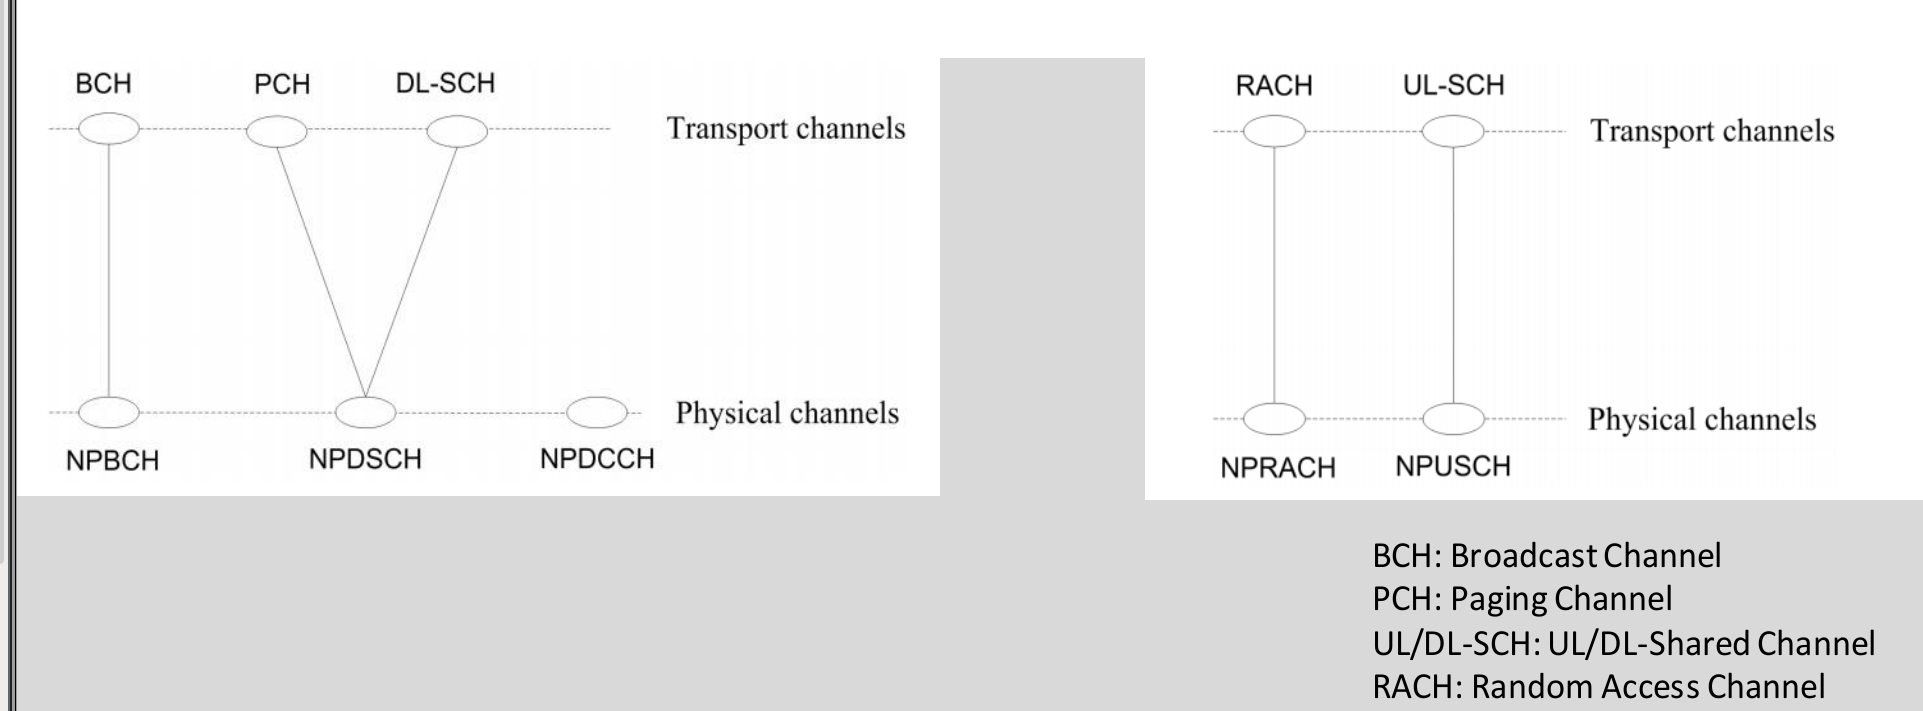
\includegraphics[width=\textwidth]{12_nbiot_transport_channels}

\subsubsection{Low-power consumption}

\paragraph{Power saving mode, PSM}

UE tells network it is going to sleep. When it intends to transmit it first
notifies the network, then remains in RX mode for 4 frames in case it needs to
be reached.'

\paragraph{Extended discontinuous reception X, eDRX}

Reduces periodicity of device to switch back to receiving mode, extends sleep
cycle ot minutes or hours. UE tells network how many hyperframes
(\SI{10.24}{\second}) it wants to sleep. Synchronization to network needed
after wakeup.
